\subsection{Principle Component Analysis}


\begin{figure}[H]
\centering
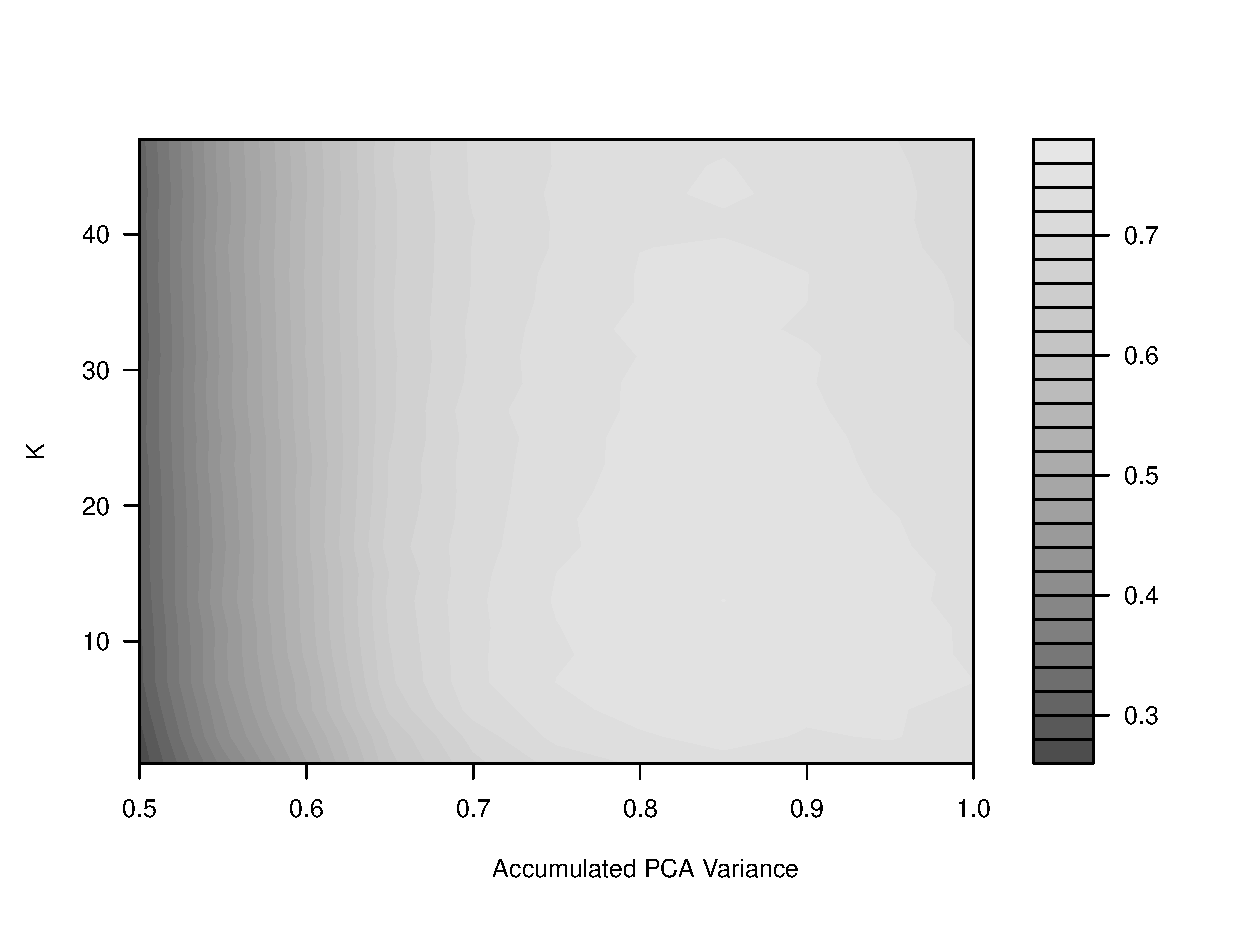
\includegraphics[width = 16cm]{graphics/contour_k_PCA_oneVsRest}
\caption{Success rate for detection of characters of Group 3 Member 2's data when he himself is not represented in the training set. 
Thewas tested with 16 people.}
\label{fig:}
\end{figure}


\begin{figure}
\centering
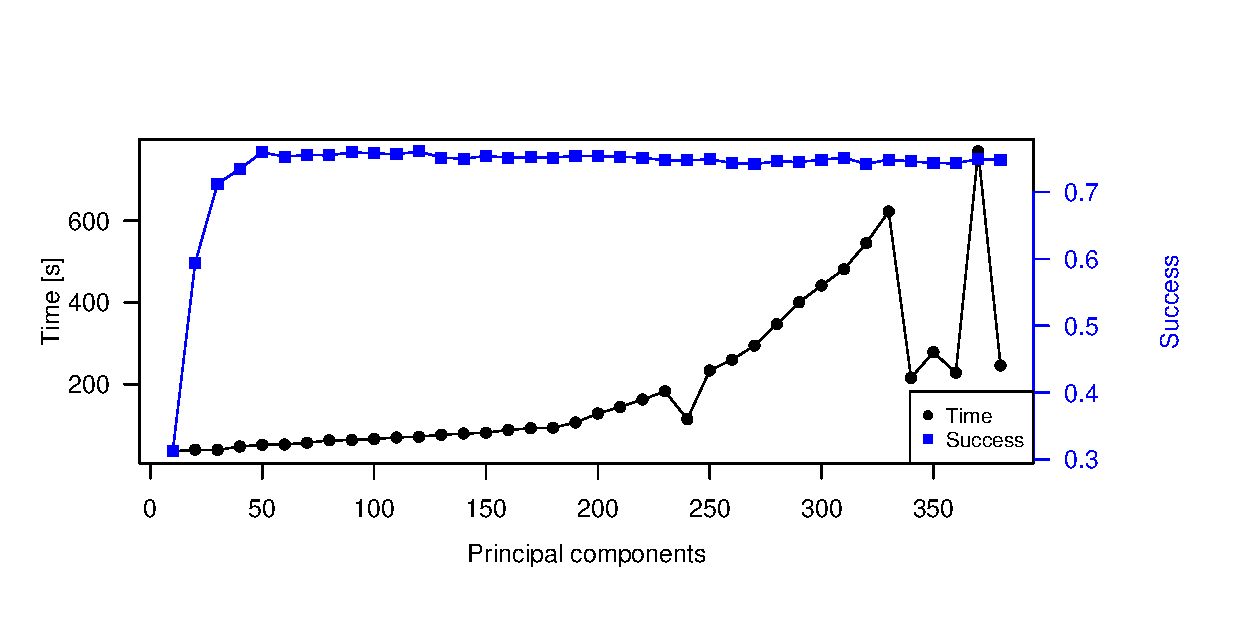
\includegraphics[width =0.8 \textwidth]{graphics/pca_timing}
\caption{Timing of running the PCA with different principle components. 
The data was run on Group 3 member 1's data on 100 DPI. 
The percentage of successful predictions is also measured with the same data.}
\label{fig:pca_timing}
\end{figure}

\begin{figure}
\centering
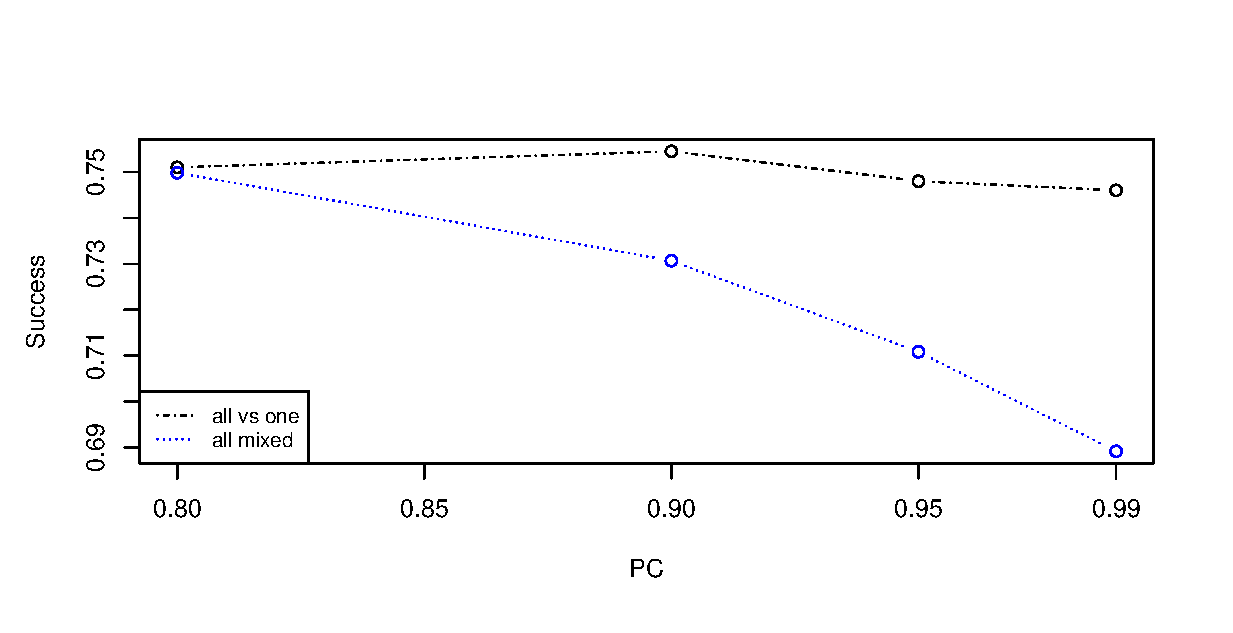
\includegraphics[width =0.8 \textwidth]{graphics/pca_success}
\caption{Percentage of successful predictions with increasing percentage of principle components used.
The data was run on Group 3 member 1's data on 100 DPI. }
\label{fig:pca_success}
\end{figure}

